\section{Theorie}
\label{sec:theo}
Die Grundlagen des Paramagnetismus, sowie die Art der Messung eben solcher Substanzen und auftretenden Problemen 
lassen sich in vier Themen unterteilen. Von besonderem Interesse ist das eigentliche Verständnis der Suszeptibilität 
auf welches im Folgenden eingegangen wird.

\subsection{Berechnung der Suszeptibilität paramagnetischer Subsatzenen}
\label{sadge1}
Ein magnetisches Feld im Vakuum kann beschrieben werden durch eine Induktionskonstante $\mu_0$ und der eigentlichen magnetischen Feldstärke
$\vec{H}$. Das Feld ist invariant, ändert sich aber wenn Matiere in das Feld reicht um den Summanden $\vec{M}$. 
\begin{equation*}
    \vec{B}=\mu_0 \vec{H} \hspace{1cm} \xrightarrow[]{\text{mit Material}} \hspace{1cm} \vec{B}=\mu_0 \vec{H} + \vec{M}
\end{equation*}
Dieser zusätzliche Term beschreibt die gemittelten magnetischen Momente der eingeführten Materie und ist wiederum propotional zum externen Feld $\vec{H}$. 
In ihm ist zudem die Suszeptibilität $\chi$ enthalten.
\begin{equation*}
    \vec{M} = \mu_0 \chi \vec{H}
\end{equation*}
Die durch $\vec{M}$ beschriebene Magnetisierung lässt sich unterscheiden zwischen Dia - und Paramagnetismus. 
Diamagnetismus liegt grundsätzlich allen Atomen bei, wobei er dem induktionerregenden, magnetischem Feld $\vec{H}$ nach der Lenzschen Regel
entegenwirkt. Folglich muss $\chi$ negativ sein.
Einige Atome besitzten zudem die Eigenschaften des Paramagnetismus, der durch einen nicht verschwindenen Drehimpuls entsteht und in einer 
Magnetisierung relativ zum externen Feld endet.
Dieses Phönomen ist auf Grund der thermischen Störung der magnetischen Momente im Gegensatz zum Diamagnetismus stark Temperatur abhängig.
Der für diese Art der Magnetisierung zentrale Drehimpuls ist dreiteilig und besteht aus dem
\begin{description}
    \item \textbf{Bahndrehimpuls} der Elektronenhülle,\\
    \item \textbf{Eigendrehimpuls} der Elektronen(auch Spin genant), \\
    \item \textbf{Kerndrehimpuls} (vernachlässigbar).
\end{description}
Es folgt nach dem Superpositionsprinzip ein Gesamtdrehimpuls $\vec{J}$ von 
\begin{equation*}
    \vec{J} = \vec{L} +\vec{S}. \hspace{2cm}\text{mit}
    \begin{cases}
        \vec{L}\text{= Gesamtbahndrehimpuls}\\
        \vec{S}\text{= Gesamtspin}\\
    \end{cases}
\end{equation*}
Die magnetischen Momente $\vec{\mu_L}$ von Gesamtbahndrehimpuls und $\vec{\mu_S}$ vom Gesamtspin sind nun beide vom Bohrschen Magneton $\mu_B$ abhängig.
Zusätzlich wird $\vec{\mu_S}$ noch durch eine weiteren Faktor $g_s$, dem gyromagnetischem Verhältnis beschrieben.
\begin{align*}
    \vec{\mu}_L &= - \frac{\vec{\mu}_B}{\hbar}\vec{L} \\
    \vec{\mu}_S &= -g_S \frac{\vec{\mu}_B}{\hbar}\vec{S} 
\end{align*}
\begin{figure}
\begin{minipage}[b]{0.5\textwidth}
Mit Hilfe der Beträge dieser Zusammenhänge lässt sich nun das gesamte magnetische Moment in Verbindung mit trigonometrischen Funktionen angeben.
Diese folgen aus der quantenmechanischen Eigenschaft, dass eben alle Impulse die nicht parallel oder antiparallel zum Gesamtbahndrehimpuls $\vec{J}$
unmessbar sind. Mit den in der Abbildung \ref{fig:winkel} gezeigten Winkeln findet sich die Formel
\begin{equation*}
    |\vec{\mu}_J| =  |\vec{\mu}_S|\text{cos}\alpha + |\vec{\mu}_L| \text{cos}\beta.
\end{equation*}
Durch Anwendung des Cosinussatzes und Benutzung vorheriger Zusammenhänge kann anschließend ein Term, bestehend aus den Quantenzahlen
der verschiedenen Impulse, gefunden werden. Der darin auftretende Bruch wird definiert als $g_J$, welcher auch Landé-Faktor genannt wird.
Mit dieser Vereinbarung reduziert sich der Betrag des gesamten magnetischen Momentes auf
\begin{equation}
    \label{eqn:idkobdasüberhaubtsstimmtlol}
    |\vec{\mu}_J| \approx |\mu_B| g_J \sqrt{J(J+1)}.
\end{equation}
\end{minipage}
\hfill
\begin{minipage}[b]{0.45\textwidth}
    \centering
    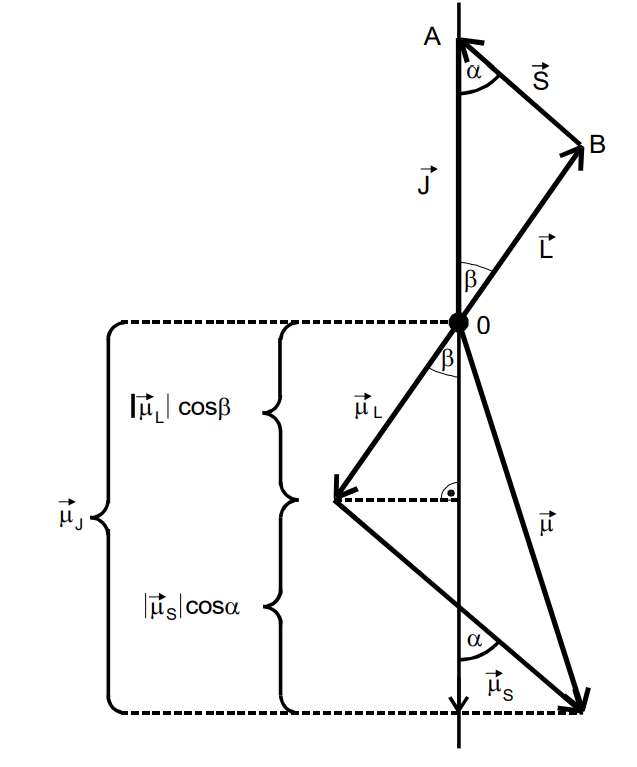
\includegraphics[width=\textwidth]{bilder/winkel.png}
    \captionsetup{justification=centering}
    \captionof{figure}{Darstellung der vektoriellen Größen\\ einer Elektronenhülle im Zweidimensionalen.\cite{skript}}
    \label{fig:winkel}
\end{minipage}
\end{figure}

Im Gegensatz zur klassischen Mechanik sind hier die möglichen Winkel stark limitiert. Die Richtungsquantelung erlaubt also nur solche Winkel, 
bei denen die Ausrichtung des Vektors $\mu_{J_z}$ von $\vec{\mu}_J$ ein Vielfaches $n \in \mathbb{N} $ von $\mu_B g_J$ ist. 
Die Quantelung für die $z$-Komponente des Gesamtbahndrehimpuls muss laso 
eine Natürliche Zahl sein und wird im folgenden $m$, Orientierungsquantenzahl genannt.
Limitierender Faktor für die Möglichkeiten von $m$ ist der Betrag von $\vec{J}$ selbst. Der Definition nach muss der 
Betrag eines Vektors stehts kleiner, oder zumindest gleich einer seiner Komponenten sein. Dadurch findet sich die Menge an 
möglichen Zahlen für $m$ als $\{-J,-J+1,...,J-1,J\}$. Jedes Element liefert eine mögliche Konfiguration des Impulses, in Summe 
bestehen also $2J+1$ Möglichkeiten. Dies wird als Zeemann-Effekt bezeichnet. Die zugehörige potentielle Energie der veschieden Einstellungen lautet
\begin{equation*}
    E_m=-|\vec{\mu}_J|\cdot\vec{B}  = \vec{\mu}_{{J_z}B}= \mu_B g_J mB.
\end{equation*}
Dabei beschreibt $g_J$ den Landé-Faktor welcher sich durch die Gleichung
\begin{equation}
    \label{eqn:landeeq}
    g_J = \frac{3J(J+1) + S(S+1) -L(L+1)}{2J(J+1)}
\end{equation}
berechnen lässt.
Die gesammelten Formeln lassen sich anschließend als Brillouin-Funktion darstellen. Diese beschreibt den gemittelten Wert 
des magnetischen Moments und somit $\chi$ in Abhängigkeit der eben definierten Impulse. Durch bestimmte Nährungen der Temperatur ergibt sich
die paramagnetische Suszeptibilität zu
\begin{equation}
    \label{eqn:CHIIII}
    \chi =  \frac{\mu_o {\mu_B}^2 {g_J}^2 N J(J+1) }{3kT},
\end{equation}
welches sich bei besonders hohen Temperatur reduzieren lässt auf die Proportionalität $\chi \sim 1 \diagup T$ was im allgemeinen
auch als das Curiesches Gesetz des Paramagnetismus bekannt ist.

\subsection{Berechnung der Suszeptibilität Seltener-Erd-Verbindungen}
\label{sadge2}
Der Bestimmung der paramagnetischen Suszeptibilität folgt nun eine Methode der Angewandten Berechnung der Suszeptibilität von 
seltenen Erden. Mit dem Hintegrund, dass diese \enquote{Erden} einen besonders hohen Paramagnetismus zeigen, bieten diese sich besonders
gut für die kommenden Messreihen an. 
\\
\newline
Mit der aufgestellten Formel \eqref{eqn:CHIIII} findet sich, dass diese Materialien also eine besonders hohe Suszeptibilität besitzen, welche 
vorallem durch den hohen Drehimpuls $J$ entsteht und auschließlich von inneren Elektronen erzeugt werden kann.
Dabei ist wichtig, dass erst die seltenen Erden ab einer Ordnungzahl $z=58$ paramagnetisches Verhalten aufweisen. 
All diese Atome besitzen Elektronen in der 4f-Schale die einen Drehimpuls erzeugen der nicht, wie bei den Vertretern mit niedrigerer
Ordnungzahl, annuliert wird. Mit Hilfe der drei Hund'schen Regeln lässt sich die genaue Anordnung der Elektronen und dadurch eben der Drehimpulse
auf diser Schale finden.
\begin{description}
    \item Nach dem Pauli-Prinzip setzt sich die Summe aller Spins $\vec{s}$ zu einem maximalen Gesamtspin $\vec{S}=\sum \vec{s_i}$ zusammen. \\
    \item Unter Einhaltung der ersten Regel und dem Pauli-Prinzip lautet der maximale Drehimpul $\vec{L}= \sum \vec{l_i}$, wobei $\vec{l_i}$ die einzelnen Drehimpulse sind.  \\
    \item Durch Kombination beider vorherigen Regeln und den Unterscheidung zwischen Schalen die weniger als halbvoll oder mehr als halbvoll sind,
    gibt es einen Gesamtbahndrehimpuls von $\vec{J} =\vec{L} \mp \vec{S}$.
\end{description}


\subsection{Beschreibung einer Apparatur zur Messung von Suszeptibilitäten}
Mit den Grundlagen aus \ref{sadge1} und \ref{sadge2} lässt sich nun eine Apparatur für das eigentliche Problem, der Bestimung 
der paramagnetischen Suszeptibilität, finden. 
Zentrales Element des Aufbaus ist eine Spule mit der entsprechenden Induktivität $L$, beschrieben durch die Anzahl ihrer Windungen $n$, Länge $l$
und dem Querschnitt $F$. 
\begin{equation}
    \label{eq:LOLLOOOOL}
    L = \mu_0 \frac{n^2}{l}F
\end{equation}
Wenn nun Materie ins Innere der Spule geschoben wird, bekommt die Formel \eqref{eq:LOLLOOOOL} zusätzlich eine Proportionalität 
$ \sim \mu$. Dieser Faktor ist abhängig von der Suszeptibilität selbst, folglich lässt sich diese dadurch mit genauen Messmitteln aus der Differenz $\Delta L$ und unter Abhängigkeit des Materialquerschnitts $Q$
bestimmen.
\begin{equation}
    \label{eqn:werdasliestistdummXD}
    \Delta L = \mu_0 \chi Q \frac{n^2}{l}
\end{equation}
\begin{figure}
\begin{minipage}{0.5\textwidth}
Um den Aufbau zu realisieren bietet es sich an, zwei Spulen mit mehreren, unter anderem variablen Widerständen zu nutzen.
Mit dem in Abbildung \ref{fig:scheißplan} gezeigten Schaltplan kann durch zwei Methoden die Suszeptibilität der eingefügten Materie gemessen werden.
Die erste Möglichkeiten ist es die auftretende Brückspannung $U_{BR}$, nach Abgleichung, zu messen. Eine Alternative dazu 
ist es nach Abgleich mit erhaltener Materie die Differenz der variablen Widerstände (vor und nach dem Abgleichen) zu messen.
\end{minipage}
\hfill
\begin{minipage}{0.4\textwidth}
    \includegraphics[width=\textwidth]{bilder/Scheiß.png}
    \captionsetup{justification=centering}
    \captionof{figure}{Schaltplan einer Brückenschaltung \\zur Messung der paramagnetischen Suszeptibilität \\ verschiedener Stoffe in zwei Möglichkeiten.\cite{skript}}
    \label{fig:scheißplan}
\end{minipage}
\end{figure}

Unter Verweundung der ersten Methode, die der Messung von der Brückenspannung findet man den Zusammenhang
%%FORMATION RUTSCHT IRGEDNWIE RUMM
\begin{equation*}
    \label{eqn:werdasliestistOMEGAdummXD}
    \chi(U_{BR})= \frac{U_{BR}}{U_{SP}} \frac{4l}{\omega \mu_0 n^2 Q} \sqrt{R^2+\omega^2 \left( \mu_0 \frac{n^2}{l}F \right)^2}.
\end{equation*}
Sollte die Frequnz $w$ hinreichend groß werden verschwindet der erste Term und die Wurzel reduziert sich auf 
\begin{equation}
    \label{eq:XD}
     \chi = 4 \frac{F}{Q}\frac{U_{BR}}{U_{SP}}.
\end{equation}
Die eben genannte Alternative gibt Aufschluss auf die Suszeptibilität unter der Abhängigkeit der Differenz des variablen Widerstands %ist zwecklos LOL
$\Delta R$. Dieser Zusammenhang beinhaltet den Widerstand $R_3$ der bekannt sein muss.
\begin{equation}
    \label{eqn:werdasliestistOMEGAundGIGAdummXD}
    \chi(\Delta R) = 2 \frac{\Delta R}{R_3}\frac{F}{Q}
\end{equation}
Dieser Aufbau gewährleistet keine problemlose Messung sondern wird verfälscht durch sogenannte Störspannungen der Brückenspannung.
Ein Selektivverstärker ist ein Bauelement in Schaltungen, welches genau die Spannungen filtern soll, die eben durch mechanische Ungenauigkeiten 
oder sonstige Störfaktoren hervorgerufen wird. Die Filterkurve ist in Abbildung \ref{fig:glocke} angegeben und hat die Gestalt einer Glockenfunktion.
\begin{figure}
    \centering
    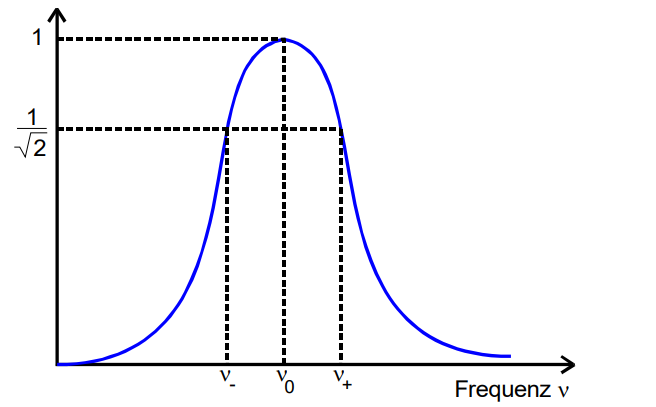
\includegraphics[width=0.5\textwidth]{bilder/glocke.png}
    \caption{lol}
    \label{fig:glocke}
\end{figure}
Die Güte $Q$ versteht sich als die Breite der Filterkurve und lässt sich wie folgt bestimmmen.
\begin{equation}
    \label{eq:achduliebeGüte}    
    Q= \frac{f_0}{f_+ - f_-}
\end{equation}
Hierbei sind $f_{\pm}$ die Abstände auf der frequnzbeschreibenden Achse, wenn die Amplitude der Kurve, also das normierte Verhältnis $U_A/U_E$,
auf $1/\sqrt{2}$ abgefallen ist.